\chapter{Micro Services Architecture} \label{chapter:MSA}
\section{Overview}
The Micro Services Architecture (MSA) is an efficient way of designing an application where suites of small services, each running its own process, communicate with each other to run a single application. Each of the services are loosely coupled and designed to work as cohesive components of a system.
Our implementation of this architecture comes with design choices for better performance of the system. Performance is discussed in the latter in this part of report. This chapter also discusses some of the disadvantages that can be observed in a micro-services architecture.
\section{Background Research}
The internet contains numerous web-applications and services that are severely limited by their interoperability. Their design promotes access to web-content rather than web services.. In an ideal world, everything should be comprised of web services, whom are all semantically labelled. This would enable an autonomous agent to discover, invoke, compose and monitor resources provided by a service. Everything on the web should be semantically clear to an automated agent so that it is able to discover, invoke, compose and monitor Web resources offering particular services and their properties \citep{martin-2004}. There is extensive research into making the Internet a more versatile platform, where applications are independent, composed and semantically meaningful. Making it possible for automated agent to execute them \citep{MSA}. Web-service architectures such as RESTful, OWL-S, WSMO, etc are some of the approaches that attempt to describe services and process the respective description enabling task automation such as execution. They often form key nodes in MSA systems. 

The Micro-services architecture is a framework to simplify the process of giving semantic meaning to the web service. Each service has a set of descriptive terms which represent a feature. For example, a feature can be a service that performs some kind of user authentication. Breaking a single application into multiple small services which focuses on performing one thing well, helps to bring that independency which is easier to provide semantic meaning to it. Not only the services are reachable from outside, it has also contributed in making a versatile system whose components can be easily replaced or upgraded without altering the whole system.

Whenever a new service is deployed, it must be described to make it available to automated agent. That requires describing its input and output semantically which details operation service performs. It is a time-consuming process and sometime ignored, however can provide great benefits. 
\section{Design}
\subsection{Design Decision}
\subsubsection{Micro-Services Architecture (MSA) vs Monolith Architecture (MA)}
Micro-Services and Monolith architecture are two different software development techniques adapted in many application building processes. MA applications are built as a single unit whereas MSA applications are composed of multiple smaller services which work together as a single unit.
Monolith architecture limits re-usability and can be confusing to group of developers to understand the core objective due to its enormity. It's not agile as it retracts from the takes away the flexibility of code when coding \citep{mulesoft_2016}.
On the other hand, MSA promotes Unix philosophy i.e. ``Do one thing and do it well''. Each service is independent, automated and self-composed which provides resiliency, agility and efficiency. Application can perform better, experience less downtime and can scale on demand \citep{mulesoft_2016}, Due to the context of making a prototype for OS and the flexibility and semantic implications of the approach, MSA is the obvious choice.
\subsubsection{HTTP 200 Error Status}
An emerging practice is returning the HTTP 200 OK status code with a Boolean `success' variable to indicate success or failure of a services request. It provides a simplicity and uniformity when dealing with errors. Notably reducing the decision tree. Application returns 200 status code using a Boolean variable `success' to indicate success or failure of the given user request. It is an emerging practice that helps to bring simplicity and uniformity when dealing with errors. It also provides a descriptive information to the client side about the incurred error. 200 status code is suitable in comparison to others as it deals with both pass and fail criteria unlike 400 error code which just notifies user about client side error.
\begin{figure}[H]
    \centering
    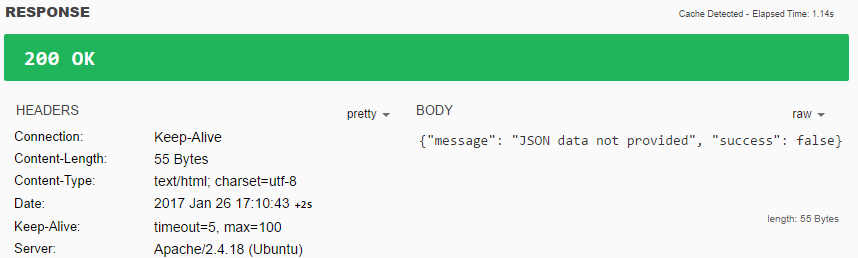
\includegraphics{figs/5/200fail}
    \caption{Screenshot of returned 200 status code}
    \label{fig:msa:200fail}
\end{figure}
\subsubsection{JSON rather than XML}
Both JSON and XML are syntaxes designed to communicate data between the server and the client side browser. Both syntaxes are human readable, hierarchical, can be parsed and used by various programming languages and can fetched using HTTP request.
But JSON outperforms XML in various ways. JSON is shorter to read and quicker to write. JSON uses array lists which provide an efficient mechanism to group all similar data. It also doesn't require a parser to be read by JavaScript programs, so it is much more compatible with front end. The use of JSON format is much simple and less prone to errors as shown in figure \ref{fig:msa:jsonvsxml} \citep{jsonvsxml}.
\begin{figure}[H]
    \centering
    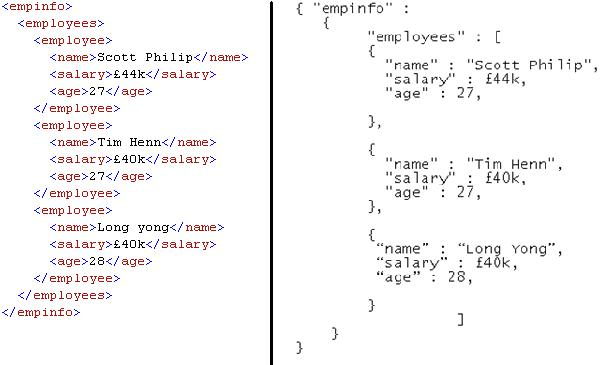
\includegraphics{figs/5/jsonvsxml}
    \caption{XML and JSON syntax format for same given data}
    \label{fig:msa:jsonvsxml}
\end{figure}
\subsubsection{Using JSON with HTTP rather than SOAP}
SOAP (Simple Object Access Protocol) is an XML based messaging protocol which sits on the top of HTTP protocol. HTTP can be considered as delivery truck which transports payload boxes packed by SOAP. Like XML, SOAP has a definite structured rule to follow making it bulky and prone to errors. Sending a JSON data via HTTP is much simpler than sending a XML data using SOAP. Not only that, SOAP is much slower in comparison as it must parse the XML file which it is embedded as payload. \citep{SOAP}
\section{Implementation}
Each micro service is a server running independently on their own personal endpoints endpoints. Flask which is a micro-framework for building python based web-servers, was used to write the server side services code. There is a route () decorator to direct services which internal function to trigger based on a given URL. It also supports WSGI (Web Server Gateway Interface) which provides an interface for back-end server to communicate with application and vice versa. \citep{introduction—wsgitutorial}
Out application implements five micro services: Productizer, Saturn, Olivia and Classifier. It also has 2 external services running as part of front end GUI. Productizer is the main client facing service that allows non-technical user input. It adds images to the SQS queue for image processing which is sends to the back-end by `Grunt' for processing. PubNub provides real time experience to the user by updating the page without having to refresh it. Communication between Productizer, SQS and Grunt take place using HTTP protocol whereas PubNub uses socket communication. This is expanded on in chapter of this report covers in more detail about the technical aspect on how front end GUI works along with two external services to handle multiple data.
All the communication between the front-end GUI and Saturn which is the main back end server, takes place using HTTP protocol (e.g. POST, GET and DELETE). Saturn is the only server that can connect front-end with the remaining two micro-services (Olivia and Classifier).
The Olivia micro-service is responsible for extracting attributes from tiled images, whereas Classifier is responsible for classifying the set of images based on their attributes. Both the servers don't have direct communication with each other. Saturn acts as a main communication tool for both.
To make each service independent and capable of operating on its own, they can handle data in both x-www-form and JSON format. All the services run on a Virtual Machine which operates on Ubuntu 16 Linux Operating System. System runs on Ubuntu because Linux provides an excellent command line command which is every useful when working with remote Virtual Machine using secure shell.
\begin{figure}[H]
    \centering
    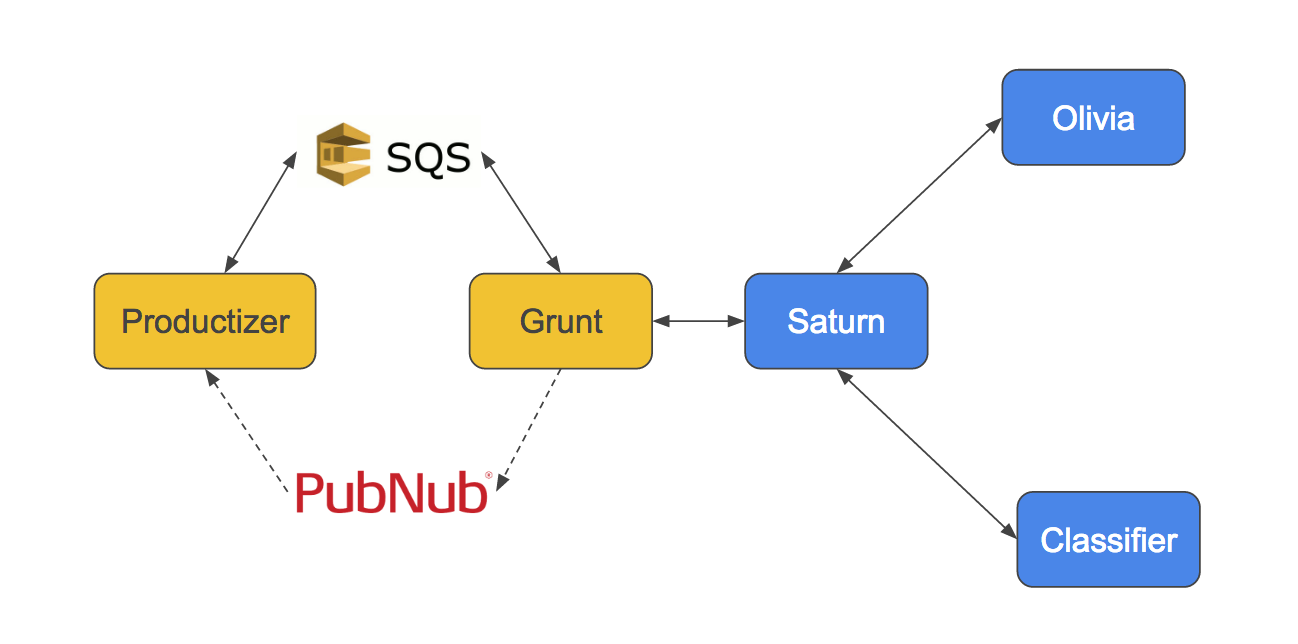
\includegraphics[width=\textwidth]{figs/5/msa}
    \caption{Application Micro-Services Architecture}
    \label{fig:msa}
\end{figure}
In figure \ref{fig:msa}, the double arrow lines represent communicate communication between micro-services using HTTP protocol whereas the dotted lines represent socket communication.
Saturn handles the data first-hand which it receives from front-end GUI. It performs necessary coordination of task in-between the micro-services and returns the data to the front end along with HTTP request status report.
\section{Testing}
For testing purposes, each endpoint was tested to see if it was active and returning the correct data. Each service has many endpoints (assessed by varying URLs), each endpoint has a different function.  So, each endpoint link was being tested to see it works, doesn't break and give out correct output using DHC (Div Http Client). DHC is an HTTP Client, well suited for API testing of multiple services. Figure \ref{fig:msa:200fail} is an example of end-point test result using DHC.
\section{Limitation}
Despite all the benefits of micro-services it is accompanied with limitations that cannot be ignored. Deploying a single application by decomposing it into multiple small services increases maintenance responsibility such as building, testing, deploying and running. Having multiple services means there must be a uniform way to communicate in between them by introducing an interface. Both sides need to exchange messages using same format and should have same understanding of message semantic.
Micro-services can be considered as a distributed system which means all the problems that exist within such system has be considered (e.g. network latency, fault tolerance, message serialisation, etc.) \citep{microservices-notafreelunch} It also increases the resource use as each service is running independently using their allocated processing power and memory. It also requires continuous monitoring as each service need to be up and running for the whole application to work. These are some of the limitations that need to be considered.
\section{Evaluation}
Micro-services architecture provides the agility to replace and update any components within the overall application. Each service can be built using the most appropriate tool for the task. Each service is small fraction of a much larger system, which can worked upon independently and at different point of time. The whole system is loosely coupled which eliminates the susceptibility of a single point of failure. In conclusion, this architecture provides this ability to work on a single application by group of people without having to worry about how the whole system works.


